\documentclass[a4paper,12pt]{book}
\usepackage[utf8]{inputenc}
\title{}
\author{Rachel Morris}
\date{\today}

\usepackage{rachwidgets}
\usepackage{fancyhdr}
\usepackage{lastpage}
\usepackage{boxedminipage}

\pagestyle{fancy}
\fancyhf{}
\lhead{CS 250}
\chead{Fall 2017}
\rhead{Lab 5: Dynamic Array Wrapper}
\rfoot{\thepage\ of \pageref{LastPage}}
\lfoot{By Rachel Morris, \footnotesize last updated \today}

\renewcommand{\headrulewidth}{2pt}
\renewcommand{\footrulewidth}{1pt}

\begin{document}

    \chapter*{Lab 5: Dynamic Array Wrapper} \stepcounter{chapter}

        \section*{Information}
            \paragraph{ Topics: } Dynamic arrays, basic data structure functionality, unit tests
            \paragraph{ Turn in: } All source files (.cpp and .hpp).
            \paragraph{ Starter files: } Download on GitHub or D2L.

\renewcommand*\DTstylecomment{\rmfamily\color{green}\textsc}

\begin{framed}
\dirtree{%
.1 Lab 05 - Dynamic Array Wrapper/.
.2 lab5\_main{.}cpp
    \dots{} \begin{minipage}[t]{5cm} Contains main() \end{minipage}.
.2 lab5\_SmartDynamicArray{.}hpp
    \dots{} \begin{minipage}[t]{5cm} Class declaration \end{minipage}.
.2 lab5\_SmartDynamicArray{.}cpp
    \dots{} \begin{minipage}[t]{5cm} Class function definitions \end{minipage}.
.2 lab5\_Tester{.}hpp
    \dots{} \begin{minipage}[t]{6cm} Unit test functions \end{minipage}.
.2 cuTEST/
    \dots{} \begin{minipage}[t]{6cm} Unit test framework \end{minipage}.
.3 Menu{.}hpp.
.3 StringUtil{.}hpp.
.3 TesterBase{.}hpp.
.3 TesterBase{.}cpp.
.2 CodeBlocks Project/.
.3 Lab 05 - Dynamic Array Wrapper{.}cbp
    \dots{} \begin{minipage}[t]{2cm}
        Code::Blocks project file
    \end{minipage}.
}
\end{framed}

Your project needs to be compiling as a C++11 project.

% ----------------------------------------------------------------------
% ----------------------------------------------------------------------
% ----------------------------------------------------------------------
    \section*{Getting started}

        This lab will be an extension of the Smart Static Array lab,
        with some changes...:

        \begin{itemize}
            \item There is no longer a MAX\_SIZE; the array can be resized.
            \item Our \texttt{m\_data} member is now a pointer, to be used
                to allocate memory for a dynamic array.
            \item We have to keep track of \texttt{m\_itemCount} as well as
                \texttt{m\_arraySize} as two integer variables now, as the array can resize.
            \item The class needs a destructor to ensure we free memory before it is destroyed.
        \end{itemize}

        A lot of the functionality will be the same, or similar to, the
        SmartStaticArray, and this lab will walk through the updates
        to make it work as a Dynamic Array wrapper.

    \subsection*{cuTEST updates}

        cuTEST has been updated so that it is not run as a console program anymore.
        Instead, it will run and immediately close after it is done, with
        the results of the unit tests written out to an html file.

        The unit test output is color coded, with failed tests highlighted in red,
        and passed tests highlighted in green. The page also contains
        descriptions for what the test tests, as well as expected and actual output values.

        \begin{center}
            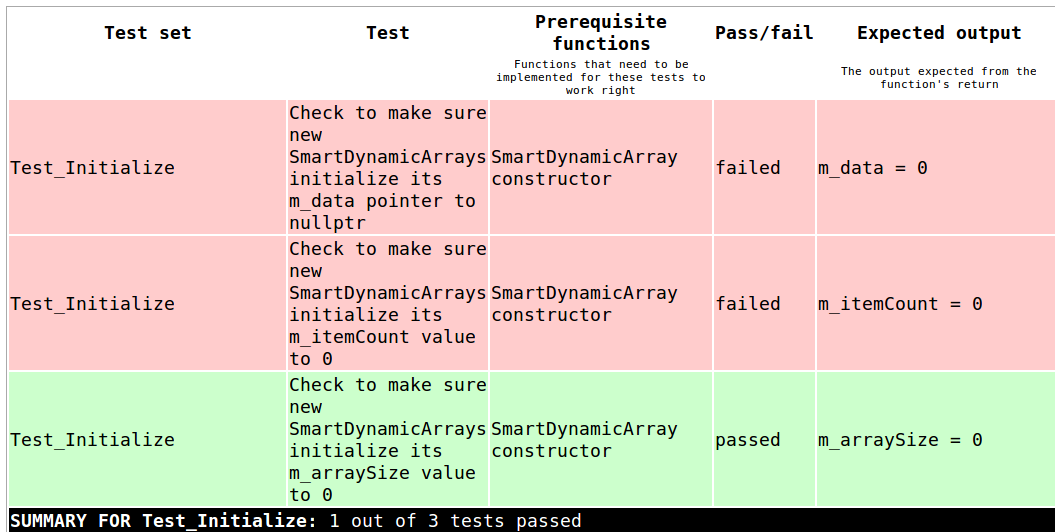
\includegraphics[width=12cm]{images/lab5-testoutput.png}
        \end{center}

        Make sure to check your project folder for the \texttt{test\_result.html} file.
        It may not be in the same location as mine, depending on what IDE you're using.
        Use your Operating System's SEARCH tool if you can't find it.

        \begin{center}
            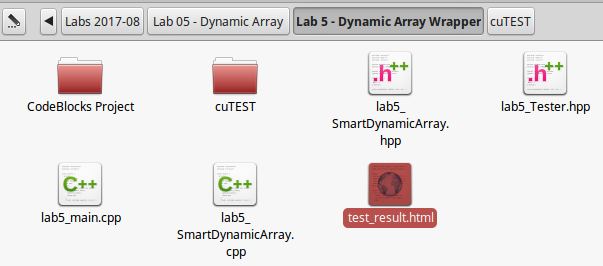
\includegraphics[width=12cm]{images/lab5-fileoutput.png}
        \end{center}



    \newpage
    \section*{The SmartDynamicArray class declaration}

        There have been some changes to the class, so let's highlight some:

\begin{lstlisting}[style=code]
class SmartDynamicArray
{
    public:
    SmartDynamicArray();
    ~SmartDynamicArray();

    void Push( const string& newItem );
    void Insert( int index, const string& newItem );
    void Extend( const SmartDynamicArray& other );
    void Pop();
    void Remove( int index );
    string Get( int index ) const;
    void Resize();
    void Resize( int newSize );

    int Size() const;
    bool IsFull() const;
    bool IsEmpty() const;

    string operator[]( int index );
    SmartDynamicArray& operator=( const SmartDynamicArray& other );
    bool operator==( const SmartDynamicArray& other );
    bool operator!=( const SmartDynamicArray& other );

    private:
    void ShiftRight( int index );
    void ShiftLeft( int index );
    bool IsInvalidIndex( int index ) const;
    bool IsNonContiguousIndex( int index ) const;
    void AllocateMemory();
    void AllocateMemory( int newSize );
    void DeallocateMemory();

    string* m_data;
    int m_itemCount;
    int m_arraySize;

    friend class Tester;
};
\end{lstlisting}

        Now for the private member variables, we have...
        \begin{verbatim}
            string* m_data
            int m_itemCount
            int m_arraySize
        \end{verbatim}

        We will be using pointers to allocate memory for a dynamic array,
        and resize it as-needed. This means we also need to take care to
        protect against memory errors.

        \begin{hint}{Need to review?}
            If you're not feeling too confident with pointers, dynamic arrays,
            and memory management, watch the video lectures for CS 200 here:

            http://edu.moosader.com/course/cs200/viewbyassignment.php
        \end{hint}

        Additionally, some of the functions added to the class are just additional
        helpers (to reduce duplicate code), or functions needed for working
        with memory management.

    \subsection*{What could possibly go wrong?}

        Some memory errors you might encounter are...

        \paragraph{Invalid Memory Address} - usually occurs when accessing
        unallocated memory, or memory that has already been freed.

        \textbf{Example 1:}

\begin{lstlisting}[style=code]
// not initialized to an address;
// pointing to garbage.
char* uninit;

// trying to de-reference the pointer.
cout << *uninit;
\end{lstlisting}

        \textbf{Example 2:}

\begin{lstlisting}[style=code]
int* listOfNumbers = new int[5]; // allocating memory
// ...(Stuff happens)...
delete [] listOfNumbers; // freeing the memory

listOfNumbers[3] = 300; // trying to access
\end{lstlisting}



        \paragraph{Memory Leaks} - occurs when memory is allocated
        but never freed.
        
        \textbf{Example:}

\begin{lstlisting}[style=code]
int main()
{
    int classSize;
    cin >> classSize;

    // Allocating memory
    string* students = new string[ classSize ];

    // No delete here!

    return 0;
}
\end{lstlisting}

        \paragraph{Missing Allocation} - occurs when you try to free
        memory that has already been freed.

        \textbf{Example:}

\begin{lstlisting}[style=code]
int main()
{
    int * myArray = new int[50];
    // (...)
    delete [] myArray;

    // later...

    delete [] myArray; // trying to free it again

    return 0;
}
\end{lstlisting}

        ~\\

        Counts will be pointed off for memory errors in ALL programs
        in this class, so make sure to be responsible with your memory management! :)

\newpage
    \section*{Implementing the functions}

        \begin{error}{Always build!}
            The unit tests provided for you will help make sure your program
            functions correctly and doesn't have logic errors, but to
            be able to \textit{use} those unit tests, your program has to
            actually build and run!

            Don't try to just implement all the functions without testing in-between,
            make sure you get one function working at a time!

            Also note that some tests have \textbf{prerequisites},
            which are listed on the test output. These are functions that
            the test relies on to function properly.
        \end{error}

        
    \subsection*{New functions}



    \subsubsection*{SmartDynamicArray()}

    \begin{framed} ~\\
        \textbf{Input parameters:} None \\
        \textbf{Return value:} None
    \end{framed}

    In this constructor, you sohuld initialize \texttt{m\_itemCount} and
    \texttt{m\_arraySize} to 0, and you should initialize the \texttt{m\_data}
    array to point to \texttt{nullptr}.

    
    % ---------------------------------------------------------------- %
    \hrulefill
    \subsubsection*{\textasciitilde SmartDynamicArray()}

    \begin{framed} ~\\
        \textbf{Input parameters:} None \\
        \textbf{Return value:} None
    \end{framed}

    In the destructor, call the \texttt{DeallocateMemory} function.

    
    % ---------------------------------------------------------------- %
    \hrulefill
    \subsubsection*{void AllocateMemory()}

    \textbf{This is an overloaded function, so there are two versions.}

    \begin{framed} ~\\
        \textbf{Input parameters:} None \\
        \textbf{Return value:} None
    \end{framed}

    Call the other version of \texttt{AllocateMemory}, passing in a default
    size value of 10.
    
    % ---------------------------------------------------------------- %
    \hrulefill
    \subsubsection*{void AllocateMemory( int newSize )}

    \textbf{This is an overloaded function, so there are two versions.}

    \begin{framed} ~\\
        \textbf{Input parameters:} newSize, an int \\
        \textbf{Return value:} None
    \end{framed}

    Use the \texttt{m\_data} pointer to create a dynamic array, if the
    pointer is not already pointing to some memory address.

    \begin{itemize}
        \item If \texttt{m\_data} is pointing to \texttt{nullptr}...
            \begin{itemize}
                \item Assign \texttt{m\_arraySize} to the value passed in as \texttt{newSize}
                \item Initialize \texttt{m\_itemCount} to 0
                \item Allocate space for a new array of size \textit{m\_arraySize} via the
                    \texttt{m\_data} pointer, and using the \textbf{new} command.            
            \end{itemize}
        \item Otherwise...
            \begin{itemize}
                \item Throw a \textbf{logic\_error} with a message that
                    memory cannot be allocated because \texttt{m\_data} is already pointing somewhere.
            \end{itemize}
    \end{itemize}
    
    % ---------------------------------------------------------------- %
    \hrulefill
    \subsubsection*{void DeallocateMemory()}

    \begin{framed} ~\\
        \textbf{Input parameters:} None \\
        \textbf{Return value:} None
    \end{framed}

    If \texttt{m\_data} is \textit{not} pointing to \texttt{nullptr}, then
    free the memory with the \textbf{delete} command, and reset the
    \texttt{m\_data} pointer to point to \texttt{nullptr}.

    
    % ---------------------------------------------------------------- %
    \newpage
    \subsubsection*{bool IsInvalidIndex( int index )}

    \begin{framed} ~\\
        \textbf{Input parameters:} some index, an integer \\
        \textbf{Return value:} None \\
        \textbf{Specifier:} This function won't throw an exception. Mark it as \texttt{noexcept}.
    \end{framed}

    Any index that is 0 or above is potentially a valid index, so this
    function only checks to see if the index passed in is less than 0.
    If the index is $< 0$, then return true - it is invalid. Otherwise,
    return false.
    
    % ---------------------------------------------------------------- %
    \hrulefill
    \subsubsection*{bool IsNonContiguousIndex( int index )}

    \begin{framed} ~\\
        \textbf{Input parameters:} some index, an integer \\
        \textbf{Return value:} None \\
        \textbf{Specifier:} This function won't throw an exception. Mark it as \texttt{noexcept}.
    \end{framed}

    An index is non-contiguous if adding an item at that index would
    cause the array to have a gap in it. For example:

    \begin{center}
        \begin{tabular}{| c | c | c | c |}
            \hline
            0 & 1 & 2 & 3
            \\ \hline
            A & B & & C
            \\ \hline
        \end{tabular}
    \end{center}

    In this case, if we allow ``C" to be inserted at position 3, then
    we will have a gap in our elements. This Dynamic Array wrapper should
    enforce the design rule that all items are next to each other.

    So, if the index is greater than the current \texttt{m\_itemCount},
    then it should return true - it is non-contiguous. Otherwise,
    return false.

    
    % ---------------------------------------------------------------- %
    \hrulefill
    \subsubsection*{void Resize()}

    \textbf{This is an overloaded function, so there are two versions.}

    \begin{framed} ~\\
        \textbf{Input parameters:} None \\
        \textbf{Return value:} None
    \end{framed}

    Call the other version of \texttt{Resize}, passing in a default
    value of the current \texttt{m\_arraySize} plus 10.


    
    
    % ---------------------------------------------------------------- %
    \newpage
    \subsubsection*{void Resize( int newSize )}

    \textbf{This is an overloaded function, so there are two versions.}

    \begin{framed} ~\\
        \textbf{Input parameters:} newSize, an integer \\
        \textbf{Return value:} None
    \end{framed}

    Follow these steps to resize the dynamic array.

    \begin{enumerate}
        \item First, check to see if \texttt{m\_data} is pointing to \texttt{nullptr}. If so:
            \begin{enumerate}
                \item Call \texttt(AllocateMemory) with the \texttt{newSize} that was passed in.
                \item Call \texttt{return} - we don't need to continue executing this function.
            \end{enumerate}

        \item Create a new dynamic array. Declare a local string-pointer variable
            and use the \textbf{new} command to create a new string array,
            whose size is \texttt{newSize}.

        \item Make for loop that iterates from 0 to \texttt{m\_arraySize} to copy items over
            from \texttt{m\_data} to your new array that you declared in step 2.

        \item Free the old memory by calling \textbf{delete \lbrack \ \rbrack} on
            the \texttt{m\_data} pointer.

        \item Update the \texttt{m\_data} pointer, and have it point to the same
            address as your new array from step 2.

        \item Update \texttt{m\_arraySize}, set it to the value of \texttt{newSize}.
    \end{enumerate}

    \begin{hint}{Confused?}
        I illustrate these steps in my Dynamic Arrays lecture from CS 200:

        http://edu.moosader.com/course/cs200/viewbyassignment.php
    \end{hint}

    
    % ---------------------------------------------------------------- %
    % ---------------------------------------------------------------- %
    % ---------------------------------------------------------------- %
    % ---------------------------------------------------------------- %

    \newpage
    \subsection*{Updated functions}

    % ---------------------------------------------------------------- %
    \subsubsection*{void Push( const string\& newItem )}

    \begin{framed} ~\\
        \textbf{Input parameters:} const string\& newItem \\
        \textbf{Return value:} None
    \end{framed}

    \paragraph{Error checking:} In this version of the array wrapper,
    we won't need to throw any exceptions from within Push. We still need
    to check for a couple of errors, and resolve them \textit{before} adding
    a new item...

    \begin{enumerate}
        \item If \texttt{m\_data} is currently pointing to \texttt{nullptr},
            then call \texttt{AllocateMemory()} before continuing.
        \item If the \texttt{IsFull()} function returns true, then call
            \texttt{Resize()} before continuing. \\
        \textbf{Specifier:} This function won't throw an exception. Mark it as \texttt{noexcept}.
    \end{enumerate}

    In both these casees, once resolved we can continue adding our new
    item as usual, so make sure your actual code to add the item to the
    array \textit{is not in an else statement}! We will add the new item
    no matter what - it's just that we needed some prep ahead of time.

    \paragraph{Store the new value:} As you did with the SmartStaticArray,
    add the new item at position \texttt{m\_itemCount} in the array,
    and make sure to increment \texttt{m\_itemCount} by 1.
    
    % ---------------------------------------------------------------- %
    \hrulefill
    \subsubsection*{bool IsFull()}

    \begin{framed} ~\\
        \textbf{Input parameters:} None \\
        \textbf{Return value:} bool, true if the array is full, or false if it is not.
    \end{framed}

    This function will now return true if \texttt{m\_itemCount} and
    \texttt{m\_arraySize} are equal values, or false if not.
    We no longer work with a MAX\_SIZE{} variable.


    % ---------------------------------------------------------------- %
    \newpage
    \subsubsection*{void Insert( int index, const string\& newItem )}

    \begin{framed} ~\\
        \textbf{Input parameters:} int index, const string\& newItem \\
        \textbf{Return value:} None
    \end{framed}

    This function will work \textit{mostly} the same as the original,
    but with one exception: If \texttt{IsFull()} returns true,
    then you call \texttt{Resize()} before continuing. This also means
    that you will remove the error check for \texttt{ index >= MAX\_SIZE }
    since there is no longer a MAX\_SIZE.




    % ---------------------------------------------------------------- %
    \hrulefill
    \subsubsection*{void Extend( const SmartStaticArray\& other )}

    \begin{framed} ~\\
        \textbf{Input parameters:} const SmartStaticArray\& other \\
        \textbf{Return value:} None
    \end{framed}

    This will work very similarly to the SmartStaticArray version,
    EXCEPT that you won't be throwing any exceptions now! If the
    size of the current array + new array is more than the current
    \texttt{m\_arraySize}, simply call \texttt{Resize(...)} before
    the extend functionality happens.

    In other words...

\begin{verbatim}
if ( m_itemCount + other.m_itemCount >= m_arraySize )
{
    Resize( m_itemCount + other.m_itemCount );
}
\end{verbatim}


    
    % ---------------------------------------------------------------- %
    % ---------------------------------------------------------------- %
    % ---------------------------------------------------------------- %
    % ---------------------------------------------------------------- %
    


    \newpage
    \subsection*{Same functionality as with SmartStaticArray}
    
    % ---------------------------------------------------------------- %
    \hrulefill
    \subsubsection*{void Pop()}

    \begin{framed} ~\\
        \textbf{Input parameters:} None \\
        \textbf{Return value:} None \\
        \textbf{Specifier:} This function won't throw an exception. Mark it as \texttt{noexcept}.
    \end{framed}

    Simply do a ``lazy-delete", and just decrement \texttt{m\_itemCount} by 1,
    if it is above 0.


    % ---------------------------------------------------------------- %
    \hrulefill
    \subsubsection*{bool IsEmpty()}

    \begin{framed} ~\\
        \textbf{Input parameters:} None \\
        \textbf{Return value:} bool, true if the array is empty, or false if it is not. \\
        \textbf{Specifier:} This function won't throw an exception. Mark it as \texttt{noexcept}.
    \end{framed}

    Just return true if the \texttt{m\_itemCount} is set to 0. Otherwise,
    return false.



    % ---------------------------------------------------------------- %
    \hrulefill
    \subsubsection*{void ShiftRight( int index )}

    \begin{framed} ~\\
        \textbf{Input parameters:} int index, the location to begin pushing items forward \\
        \textbf{Return value:} None \\
        \textbf{Specifier:} This function won't throw an exception. Mark it as \texttt{noexcept}.
    \end{framed}

    Every element at the given index and after it should be shifted right by one space.
    

    % ---------------------------------------------------------------- %
    \newpage
    \subsubsection*{void ShiftLeft( int index )}

    \begin{framed} ~\\
        \textbf{Input parameters:} int index, the location to begin pulling items backwards \\
        \textbf{Return value:} None \\
        \textbf{Specifier:} This function won't throw an exception. Mark it as \texttt{noexcept}.
    \end{framed}

    Every element at the given index and after it should be shifted left by one space.


    % ---------------------------------------------------------------- %
    \hrulefill
    \subsubsection*{int Size()}

    \begin{framed} ~\\
        \textbf{Input parameters:} None \\
        \textbf{Return value:} int, the amount of items stored in the array. \\
        \textbf{Specifier:} This function won't throw an exception. Mark it as \texttt{noexcept}.
    \end{framed}

    This function will only return the current value of the
    private member variable, \texttt{m\_itemCount}.


    % ---------------------------------------------------------------- %
    \hrulefill
    \subsubsection*{string Get( int index )}

    \begin{framed} ~\\
        \textbf{Input parameters:} int index \\
        \textbf{Return value:} string, the value from the array
    \end{framed}

    If the index is invalid (less than 0, or greater than or equal to
    the \texttt{m\_itemCount}), then throw an \textbf{out\_of\_range}
    exception.

    Otherwise, return the element from \texttt{m\_data} at the \texttt{index}
    passed in.




    % ---------------------------------------------------------------- %
    \newpage
    \subsubsection*{void Remove( int index )}

    \begin{framed} ~\\
        \textbf{Input parameters:} None \\
        \textbf{Return value:} None
    \end{framed}

    \paragraph{Error checking:}
    Check to see if the index is invalid (less than 0 or greater than
    or equal to \texttt{m\_itemCount}). If it is invalid, then
    \textbf{throw} an \texttt{out\_of\_range} exception
    with the message, ``Cannot insert at index - out of range".

    \paragraph{Functionality:}
    If there is no exception thrown, then call the \texttt{ShiftLeft}
    function, passing in the index. Again, we are \textit{lazy deleting}
    the data by simply overwriting it with this function call.

    Afterwards, make sure to decrement \texttt{m\_itemCount}.



\newpage
\section*{Grading breakdown}

\begin{tabular}{ | p{8cm} | p{4cm} | }
    \hline
    \textbf{Function} & \textbf{Point value}
    \\ \hline

    SmartDynamicArray constructor       & 3
    \\ \hline
    SmartDynamicArray destructor        & 3
    \\ \hline

    AllocateMemory functions            & 4
    \\ \hline
    DeallocateMemory                    & 3
    \\ \hline

    IsInvalidIndex                      & 1
    \\ \hline
    IsNonContiguousIndex                & 1
    \\ \hline

    Resize functions                    & 8
    \\ \hline


    Push                                & 2
    \\ \hline
    IsFull                              & 1
    \\ \hline
    Insert                              & 2
    \\ \hline
    Extend                              & 2
    \\ \hline

    
    
    & \\ \hline
    \textbf{Total} & 30
    \\ \hline
\end{tabular}


\end{document}









